% !TeX program = lualatex
% ================================================================
% Polish Parallel Text Version of LatticeMethod
%
% Generated by the server using the following settings:
%
%   language            Polish (pol)
%   text direction      left to right
%   font                Noto Serif
%   fallback font       Noto Serif
%   built from          latex/slides/latticeMethod.tex
%   vocabulary key      latex/slides/latticeMethod/L2/pol/latticeMethod_polishKey.tex
%   tier 3 vocabulary   green   RGB 0 128 0
%   English text        black   RGB 0 0 0
%   Polish text         purple  RGB 112 48 160
%   layout macros       version 3
%
% Please don't edit any information in this comment block - the server
% compares it against the current settings and rebuilds this file when
% they differ, so changes here would be overwritten. However, feel free
% to make updates to the LaTeX below if you want to edit it.
% ================================================================

\documentclass[10pt,aspectratio=169]{beamer}
% ================================================================
% Copied from the English sheet this was translated from, so that
% anything it sets up for itself still works here
% ================================================================
\usepackage[T1]{fontenc}
%\usepackage{lmodern} % not installed here; safe to re-enable locally
\usepackage{amsmath,amssymb}
\usepackage{array,colortbl}
\usepackage{tikz}
\usetikzlibrary{calc,positioning,arrows.meta,decorations.pathreplacing}

\usetheme{default}
\usecolortheme{default}
\setbeamertemplate{navigation symbols}{}
\setbeamertemplate{itemize items}[circle]

%--------------------------------------------------- colours
\definecolor{mmblue}{RGB}{28,77,120}
\definecolor{mmred}{RGB}{176,42,55}
\definecolor{mmgreen}{RGB}{35,110,75}
\definecolor{mmgrey}{RGB}{120,120,120}
\definecolor{bandA}{RGB}{255,232,200}   % units      diagonal
\definecolor{bandB}{RGB}{212,233,246}   % tens       diagonal
\definecolor{bandC}{RGB}{225,243,220}   % hundreds   diagonal
\definecolor{bandD}{RGB}{238,225,243}   % thousands  diagonal

\setbeamercolor{frametitle}{fg=white,bg=mmblue}
\setbeamercolor{title}{fg=mmblue}
\setbeamercolor{structure}{fg=mmblue}
\setbeamerfont{frametitle}{series=\bfseries}
\setbeamertemplate{frametitle}{%
  \vspace*{2pt}\hspace*{6pt}\insertframetitle\vspace*{3pt}}

%--------------------------------------------------- answer overlay
% If your own preamble already defines these, yours are used instead.
\providecommand{\ablank}[1]{\uncover<2->{\textcolor{mmred}{#1}}}
\providecommand{\ashow}[1]{\textcolor{mmred}{#1}}

%--------------------------------------------------- lattice toolkit
\tikzset{
  cellline/.style={draw=mmblue,line width=0.7pt},
  diagline/.style={draw=mmblue!60,line width=0.6pt},
  headfont/.style={font=\bfseries},
}

% \lgrid{cols}{rows} : boxes + diagonals
\newcommand{\lgrid}[2]{%
  \foreach \c in {1,...,#1}{%
    \foreach \r in {1,...,#2}{%
      \draw[cellline] ({\c-1},{-\r+1}) rectangle ({\c},{-\r});
      \draw[diagline] ({\c},{-\r+1}) -- ({\c-1},{-\r});}}%
}

% \lband{cols}{rows}{a}{colour} : shade the strip a <= x-y <= a+1
\newcommand{\lband}[4]{%
  \begin{scope}
    \clip (0,0) rectangle ({#1},{-#2});
    \fill[#4] ({#3},0) -- ({#3+1},0) -- ({#3-7},-8) -- ({#3-8},-8) -- cycle;
  \end{scope}%
}

% \ldiag{cols}{rows}{a}{colour} : draw the diagonal line x-y = a, extended
\newcommand{\ldiag}[4]{%
  \begin{scope}
    \clip ({-0.6},0.0) rectangle ({#1},{-#2-0.6});
    \draw[#4,line width=1.4pt] ({#3+1},1) -- ({#3-8},-8);
  \end{scope}%
}

% \ltop{col}{digit}  column heading
\newcommand{\ltop}[2]{\node[headfont] at ({#1-0.5},{0.32}) {#2};}
% \lside{cols}{row}{digit}  row heading on the right
\newcommand{\lside}[3]{\node[headfont] at ({#1+0.35},{-#2+0.5}) {#3};}
% \lcell{col}{row}{tens}{units}
\newcommand{\lcell}[4]{%
  \node at ({#1-0.72},{-#2+0.70}) {\small #3};
  \node at ({#1-0.28},{-#2+0.30}) {\small #4};}
% \lleft{row}{digit}  answer digit at left edge
\newcommand{\lleft}[2]{\node[mmred,font=\bfseries] at ({-0.42},{-#1+0.5}) {#2};}
% \lbot{cols}{rows}{col}{digit} answer digit under the bottom edge
\newcommand{\lbot}[4]{\node[mmred,font=\bfseries] at ({#3-0.5},{-#2-0.42}) {#4};}

%--------------------------------------------------- misc
\newcommand{\hl}[1]{\textcolor{mmred}{#1}}
\newcommand{\gd}[1]{\textcolor{mmgreen}{#1}}
\renewcommand{\arraystretch}{1.35}

\title{Lattice Multiplication}
\subtitle{From rectangles, to grids, to diagonals}
\author{}
\date{}

% Characters this language's font has not got are borrowed from another,
% rather than being silently dropped - see docs/translated-sheet-latex.md
\directlua{%
  if luaotfload and luaotfload.add_fallback then
    luaotfload.add_fallback("eallatinfallback",
      { "Noto Serif:mode=harf;" })
  else
    tex.error("this luaotfload is too old to register a fallback font")
  end
}
\usepackage[english]{babel}
\babelprovide[import]{polish}
\babelfont[polish]{rm}[Renderer=Harfbuzz, BoldFont={Noto Serif}, ItalicFont={Noto Serif}, BoldItalicFont={Noto Serif}, RawFeature={fallback=eallatinfallback}]{Noto Serif}
\babelfont[polish]{sf}[Renderer=Harfbuzz, BoldFont={Noto Serif}, ItalicFont={Noto Serif}, BoldItalicFont={Noto Serif}, RawFeature={fallback=eallatinfallback}]{Noto Serif}
\newcommand{\ealtext}[1]{\foreignlanguage{polish}{#1}}
\newcommand{\ealtextblock}[1]{{\raggedright\foreignlanguage{polish}{#1}\par}}
% ================================================================
% EAL layout helpers
% ================================================================
\usepackage{xcolor}

\definecolor{ealkeycolour}{RGB}{0,128,0}
\definecolor{ealenglish}{RGB}{0,0,0}
\definecolor{ealtwocolour}{RGB}{112,48,160}

\newsavebox{\ealboxen}
\newsavebox{\ealboxtr}
\newlength{\ealglosswd}
\newlength{\ealglossraise}
\setlength{\ealglossraise}{1.15em}

% a tier 3 word, in English and in translation alike
\newcommand{\ealkey}[1]{\textcolor{ealkeycolour}{#1}}
\newcommand{\ealkeytr}[1]{\textcolor{ealkeycolour}{\ealtext{#1}}}

% One translated word above one English word. Built from kernel
% primitives, never a tabular, which would break wherever the sheet
% loads array, booktabs or tabularx. The box is as wide as the wider of
% the two, so a long translation pushes its neighbours aside instead of
% overlapping them, and it claims its full height so a table row or a
% TikZ node makes room for it.
\newcommand{\ealgloss}[2]{%
  \sbox{\ealboxen}{\ealkey{#1}}%
  \sbox{\ealboxtr}{\small\textcolor{ealtwocolour}{\ealtext{#2}}}%
  \setlength{\ealglosswd}{\wd\ealboxen}%
  \ifdim\wd\ealboxtr>\ealglosswd\setlength{\ealglosswd}{\wd\ealboxtr}\fi
  \leavevmode
  \makebox[\ealglosswd][c]{%
    \makebox[0pt][c]{\usebox{\ealboxen}}%
    \makebox[0pt][c]{\raisebox{\ealglossraise}{\usebox{\ealboxtr}}}%
  }%
}

% opens up line spacing around a block of glosses, so the raised
% translations sit clear of the line above
\newenvironment{ealglossed}{\par\linespread{2.1}\selectfont\ignorespaces}{\par}

% a whole translated sentence above its English counterpart. block level,
% so it does not belong inside a tabular cell
\newcommand{\ealpara}[2]{%
  \par\addvspace{0.5\baselineskip}%
  {\color{ealtwocolour}\ealtextblock{#1}}%
  \penalty200
  {\color{ealenglish}#2\par}%
  \addvspace{0.5\baselineskip}%
}

\begin{document}

%=====================================================================
\begin{frame}[plain]
  \vfill
  \centering
  \ealpara{\ealkeytr{Krata} \ealkeytr{mnożenie}}{\ealkey{Lattice} \ealkey{Multiplication}}
  \vspace{4pt}
  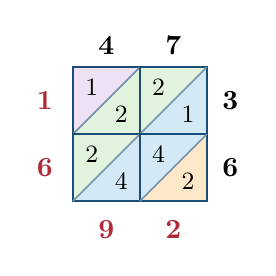
\begin{tikzpicture}[scale=0.85]
    \lband{2}{2}{3}{bandA}\lband{2}{2}{2}{bandB}
    \lband{2}{2}{1}{bandC}\lband{2}{2}{0}{bandD}
    \lgrid{2}{2}
    \ltop{1}{4}\ltop{2}{7}\lside{2}{1}{3}\lside{2}{2}{6}
    \lcell{1}{1}{1}{2}\lcell{2}{1}{2}{1}
    \lcell{1}{2}{2}{4}\lcell{2}{2}{4}{2}
    \lleft{1}{1}\lleft{2}{6}\lbot{2}{2}{1}{9}\lbot{2}{2}{2}{2}
  \end{tikzpicture}
  \vfill
\end{frame}

%=====================================================================
\begin{frame}
  \ealpara{Dokąd zmierzamy}{Where we are going}
  \vspace{6pt}
  \begin{columns}[T]
    \begin{column}{0.33\textwidth}
      \centering
      \ealpara{1. \ealkeytr{Pole}}{1. \ealkey{Area}}
      \vspace{6pt}
      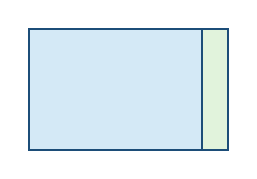
\begin{tikzpicture}[scale=0.11]
        \fill[bandB] (0,0) rectangle (20,14);
        \fill[bandC] (20,0) rectangle (23,14);
        \draw[mmblue,thick] (0,0) rectangle (23,14);
        \draw[mmblue] (20,0) -- (20,14);
      \end{tikzpicture}
      \vspace{6pt}
      \ealpara{Mnożenie to znajdowanie \ealkeytr{pola} \ealkeytr{prostokąta}.}{Multiplying is finding the \ealkey{area} of a \ealkey{rectangle}.}
    \end{column}
    \begin{column}{0.33\textwidth}
      \centering
      \ealpara{2. Metoda \ealkeytr{siatki}}{2. \ealkey{Grid} method}
      \vspace{6pt}
      {\footnotesize
      \begin{tabular}{|c|c|c|}\hline
        $\times$ & $20$ & $3$\\\hline
        $10$ & $200$ & $30$\\\hline
        $4$ & $80$ & $12$\\\hline
      \end{tabular}}
      \vspace{6pt}
      \ealpara{\ealkeytr{Prostokąt} zapisany jako tabela. Każde zero pokazane.}{The \ealkey{rectangle} written as a table. Every zero shown.}
    \end{column}
    \begin{column}{0.33\textwidth}
      \centering
      \ealpara{3. \ealkeytr{Krata}}{3. \ealkey{Lattice}}
      \vspace{6pt}
      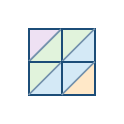
\begin{tikzpicture}[scale=0.42]
        \lband{2}{2}{3}{bandA}\lband{2}{2}{2}{bandB}
        \lband{2}{2}{1}{bandC}\lband{2}{2}{0}{bandD}
        \lgrid{2}{2}
      \end{tikzpicture}
      \vspace{6pt}
      \ealpara{Te same \ealkeytr{iloczyny}, z \ealkeytr{przekątnymi} wykonującymi \ealkeytr{wartość pozycyjną}.}{The same \ealkey{products}, with the \ealkey{diagonals} doing the \ealkey{place value}.}
    \end{column}
  \end{columns}
  \vspace{10pt}
\end{frame}

%=====================================================================
\begin{frame}
  \ealpara{\ealkeytr{Mnożenie} to \ealkeytr{pole}}{\ealkey{Multiplication} is \ealkey{area}}
  \vspace{6pt}
  \begin{columns}[c]
    \begin{column}{0.5\textwidth}
      \centering
      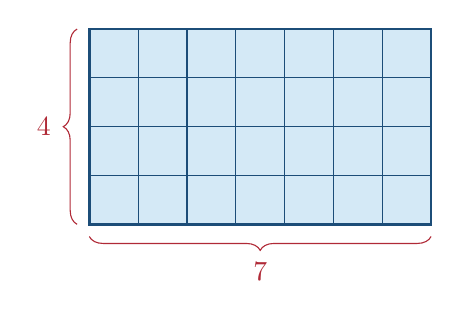
\begin{tikzpicture}[scale=0.62]
        \fill[bandB] (0,0) rectangle (7,4);
        \draw[mmblue,step=1] (0,0) grid (7,4);
        \draw[mmblue,line width=1pt] (0,0) rectangle (7,4);
        \draw[decorate,decoration={brace,amplitude=5pt,mirror},mmred]
              (0,-0.25) -- (7,-0.25) node[midway,below=6pt]{$7$};
        \draw[decorate,decoration={brace,amplitude=5pt},mmred]
              (-0.25,0) -- (-0.25,4) node[midway,left=6pt]{$4$};
      \end{tikzpicture}
    \end{column}
    \begin{column}{0.5\textwidth}
      \begin{itemize}
        \item \ealpara{\ealkeytr{Prostokąt} o szerokości $7$ i wysokości $4$.}{A \ealkey{rectangle} $7$ wide and $4$ tall.}
        \item \ealpara{Policz \ealkeytr{kwadraty}: $7 \times 4 = 28$.}{Count the \ealkey{squares}: $7 \times 4 = 28$.}
        \item[] \ealpara{Każde pytanie o \ealkeytr{mnożenie} można przedstawić jako \ealkeytr{prostokąt}.}{Every \ealkey{multiplication} question can be represented as a \ealkey{rectangle}.}
      \end{itemize}
    \end{column}
  \end{columns}
\end{frame}

%=====================================================================
\begin{frame}
  \ealpara{Pocięcie \ealkeytr{prostokąta}}{Chopping the \ealkey{rectangle} up}
  \vspace{6pt}
  \begin{center}
    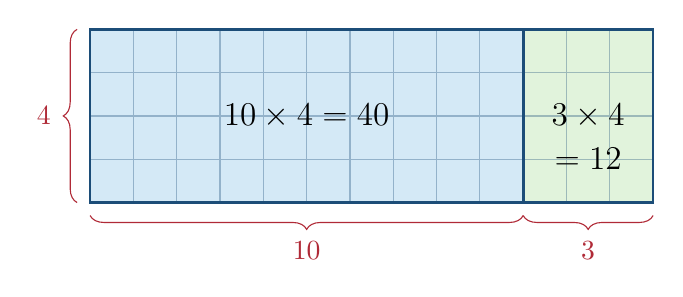
\begin{tikzpicture}[scale=0.55]
      \fill[bandB] (0,0) rectangle (10,4);
      \fill[bandC] (10,0) rectangle (13,4);
      \draw[mmblue,step=1,opacity=0.35] (0,0) grid (13,4);
      \draw[mmblue,line width=1pt] (0,0) rectangle (13,4);
      \draw[mmblue,line width=1.2pt] (10,0) -- (10,4);
      \node at (5,2) {\large $10\times 4 = 40$};
      \node at (11.5,2) {\large $3\times 4$};
      \node at (11.5,1) {\large $=12$};
      \draw[decorate,decoration={brace,amplitude=5pt,mirror},mmred]
            (0,-0.3) -- (10,-0.3) node[midway,below=6pt]{$10$};
      \draw[decorate,decoration={brace,amplitude=5pt,mirror},mmred]
            (10,-0.3) -- (13,-0.3) node[midway,below=6pt]{$3$};
      \draw[decorate,decoration={brace,amplitude=5pt},mmred]
            (-0.3,0) -- (-0.3,4) node[midway,left=6pt]{$4$};
    \end{tikzpicture}
  \end{center}
  \vspace{-4pt}
  \begin{center}
    \large $13 \times 4 \;=\; (10\times 4) + (3\times 4) \;=\; 40 + 12 \;=\; \hl{52}$
  \end{center}
  \vspace{4pt}
  \ealpara{Dzielimy $13$ na części, które możemy faktycznie pomnożyć w głowie: jej \ealkeytr{dziesiątki} i \ealkeytr{jedności}.}{We split $13$ into the parts we can actually multiply in our heads: its \emph{\ealkey{tens}} and its \emph{\ealkey{units}}.}
\end{frame}

%=====================================================================
\begin{frame}
  \ealpara{Dwie \ealkeytr{cyfry} przez dwie \ealkeytr{cyfry}: cztery części}{Two \ealkey{digits} by two \ealkey{digits}: four pieces}
  \vspace{6pt}
  \begin{center}
    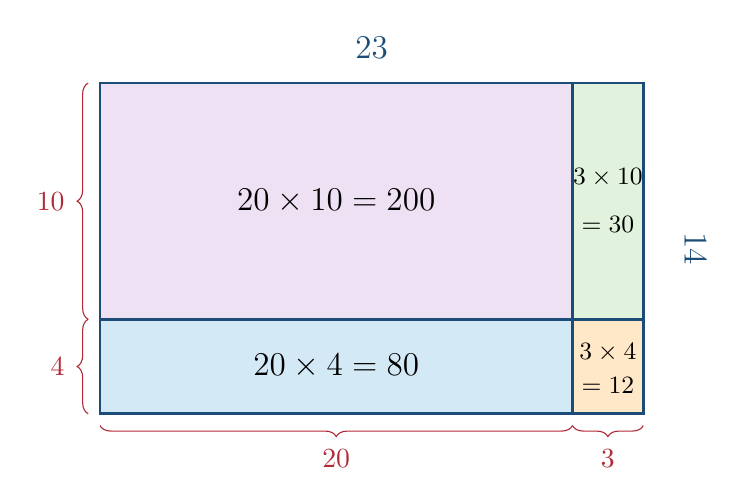
\begin{tikzpicture}[scale=0.30]
      \fill[bandD] (0,4) rectangle (20,14);
      \fill[bandC] (20,4) rectangle (23,14);
      \fill[bandB] (0,0) rectangle (20,4);
      \fill[bandA] (20,0) rectangle (23,4);
      \draw[mmblue,line width=1pt] (0,0) rectangle (23,14);
      \draw[mmblue,line width=1.2pt] (20,0) -- (20,14);
      \draw[mmblue,line width=1.2pt] (0,4) -- (23,4);
      \node at (10,9)   {\large $20\times 10 = 200$};
      \node at (21.5,10) {\small $3\times 10$};
      \node at (21.5,8)  {\small $=30$};
      \node at (10,2)   {\large $20\times 4 = 80$};
      \node at (21.5,2.6) {\small $3\times4$};
      \node at (21.5,1.2) {\small $=12$};
      \draw[decorate,decoration={brace,amplitude=4pt,mirror},mmred]
            (0,-0.5) -- (20,-0.5) node[midway,below=5pt]{$20$};
      \draw[decorate,decoration={brace,amplitude=4pt,mirror},mmred]
            (20,-0.5) -- (23,-0.5) node[midway,below=5pt]{$3$};
      \draw[decorate,decoration={brace,amplitude=4pt},mmred]
            (-0.5,4) -- (-0.5,14) node[midway,left=5pt]{$10$};
      \draw[decorate,decoration={brace,amplitude=4pt},mmred]
            (-0.5,0) -- (-0.5,4) node[midway,left=5pt]{$4$};
      \node[mmblue] at (11.5,15.5) {\large\bfseries $23$};
      \node[mmblue,rotate=-90] at (25.2,7) {\large\bfseries $14$};
    \end{tikzpicture}
  \end{center}
  \vspace{-2pt}
  \begin{center}
    \large $23\times 14 \;=\; 200 + 30 + 80 + 12 \;=\; \hl{322}$
  \end{center}
\end{frame}

%=====================================================================
\begin{frame}
  \ealpara{Ten sam \ealkeytr{prostokąt}, zapisany jako \ealkeytr{siatka}}{The same \ealkey{rectangle}, written as a \ealkey{grid}}
  \vspace{6pt}
  \begin{columns}[c]
    \begin{column}{0.46\textwidth}
      \centering
      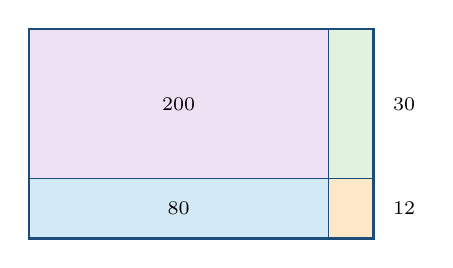
\begin{tikzpicture}[scale=0.19]
        \fill[bandD] (0,4) rectangle (20,14);
        \fill[bandC] (20,4) rectangle (23,14);
        \fill[bandB] (0,0) rectangle (20,4);
        \fill[bandA] (20,0) rectangle (23,4);
        \draw[mmblue,line width=1pt] (0,0) rectangle (23,14);
        \draw[mmblue] (20,0) -- (20,14);
        \draw[mmblue] (0,4) -- (23,4);
        \node[font=\scriptsize] at (10,9) {$200$};
        \node[font=\scriptsize] at (10,2) {$80$};
        \node[font=\scriptsize,right=1pt] at (23.5,9) {$30$};
        \node[font=\scriptsize,right=1pt] at (23.5,2) {$12$};
      \end{tikzpicture}
    \end{column}
    \begin{column}{0.10\textwidth}
      \centering{\Huge\color{mmblue}$\Rightarrow$}
    \end{column}
    \begin{column}{0.42\textwidth}
      \centering
      \begin{tabular}{|c|c|c|}\hline
        \bfseries $\times$ & \bfseries $20$ & \bfseries $3$\\\hline
        \bfseries $10$ & \cellcolor{white}$200$ & $30$\\\hline
        \bfseries $4$ & $80$ & $12$\\\hline
      \end{tabular}\\[10pt]
      {\small $200+30+80+12 = \hl{322}$}
    \end{column}
  \end{columns}
  \vspace{8pt}
  \begin{itemize}
    \item \ealpara{\ealkeytr{Siatka} jest jak obrazek, ale nie jest narysowana w skali.}{The \ealkey{grid} is like the picture, but not drawn to scale.}
  \end{itemize}
\end{frame}

%=====================================================================
\begin{frame}
  \ealpara{Zachowaj każde zero}{Keep every zero}
  \vspace{6pt}
  \begin{center}
    \begin{tabular}{|c|c|c|}\hline
      \bfseries $\times$ & \bfseries $40$ & \bfseries $7$\\\hline
      \bfseries $30$ & $1200$ & $210$\\\hline
      \bfseries $6$  & $240$  & $42$\\\hline
    \end{tabular}
    \hspace{18pt}
    \begin{minipage}{0.42\textwidth}
      \begin{align*}
        4\times 3 &= 12 &&\text{so } \hl{40}\times \hl{30} = \hl{1200}\\
        4\times 6 &= 24 &&\text{so } \hl{40}\times 6 = \hl{240}\\
        7\times 3 &= 21 &&\text{so } 7\times \hl{30} = \hl{210}\\
        7\times 6 &= 42 &&\text{so } 7\times 6 = 42
      \end{align*}
    \end{minipage}
  \end{center}
  \vspace{4pt}
  \begin{center}
    \ealpara{$1200+240+210+42 = 1692$, więc $47\times 36 = 1692$}{$1200+240+210+42 = 1692$, so $47\times 36 = 1692$}
  \end{center}
  \vspace{4pt}
\end{frame}

%=====================================================================
\begin{frame}
  \ealpara{Twoja kolej: metoda \ealkeytr{siatki}}{Your turn: \ealkey{grid} method}
  \vspace{6pt}
  \begin{center}
    \begin{tabular}{lll}
      \textbf{(a)} $34\times 12 = \ablank{408}$ &\quad
      \textbf{(b)} $26\times 45 = \ablank{1170}$ &\quad
      \textbf{(c)} $53\times 27 = \ablank{1431}$\\[10pt]
      \textbf{(d)} $18\times 63 = \ablank{1134}$ &\quad
      \textbf{(e)} $72\times 84 = \ablank{6048}$ &\quad
      \textbf{(f)} $95\times 48 = \ablank{4560}$
    \end{tabular}
  \end{center}
  \vspace{10pt}
  \begin{center}
    \begin{tabular}{|c|c|c|}\hline
      \bfseries $\times$ & & \\\hline
      & & \\\hline
      & & \\\hline
    \end{tabular}
    \hspace{20pt}
    \begin{minipage}{0.45\textwidth}
      \ealpara{\textbf{Wyzwanie.} $124 \times 36$. Ile pól potrzebuje teraz twoja \ealkeytr{siatka} i dlaczego?}{\textbf{Challenge.} $124 \times 36$. How many boxes does your \ealkey{grid} need now, and why?}
      \vspace{4pt}
      \ealpara{Odpowiedź: \ablank{$3\times 2 = 6$ pól, po jednym dla każdej pary \ealkeytr{wartości pozycyjnych}; $124\times 36 = 4464$}}{Answer: \ablank{$3\times 2 = 6$ boxes, one for each pair of \ealkey{place value}s; $124\times 36 = 4464$}}
    \end{minipage}
  \end{center}
\end{frame}

%=====================================================================
\begin{frame}
  \ealpara{Problem z \ealkeytr{siatką}}{The problem with the \ealkey{grid}}
  \vspace{6pt}
  \begin{center}
    \begin{tabular}{|c|c|c|c|}\hline
      \bfseries $\times$ & \bfseries $300$ & \bfseries $40$ & \bfseries $7$\\\hline
      \bfseries $600$ & $180000$ & $24000$ & $4200$\\\hline
      \bfseries $50$  & $15000$  & $2000$  & $350$\\\hline
      \bfseries $8$   & $2400$   & $320$   & $56$\\\hline
    \end{tabular}
  \end{center}
  \vspace{8pt}
  \begin{itemize}
    \item \ealpara{Metoda jest dobra dla większych liczb...}{The method is fine for bigger numbers...}
    \item \ealpara{Ale to dużo pisania długich liczb}{But it is a lot of writing long numbers}
    \item[] \ealpara{\ealkeytr{Krata} zachowuje te same dziewięć \ealkeytr{iloczynów}, ale zapisuje tylko \ealkeytr{cyfry} --- i używa \ealkeytr{przekątnych} zamiast zer, aby śledzić \ealkeytr{wartość pozycyjną}.}{\ealkey{Lattice} keeps the same nine \ealkey{products} but writes only the \ealkey{digits} --- and uses \emph{\ealkey{diagonals}} instead of zeros to keep track of \ealkey{place value}.}
  \end{itemize}
\end{frame}

%=====================================================================
\begin{frame}
  \ealpara{Budowanie \ealkeytr{kraty}: krok 1, narysuj ją}{Building a \ealkey{lattice}: step 1, draw it}
  \vspace{6pt}
  \begin{columns}[c]
    \begin{column}{0.45\textwidth}
      \centering
      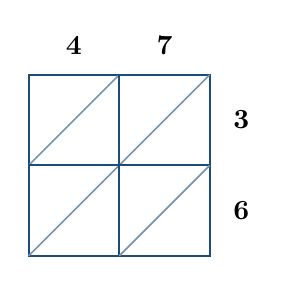
\begin{tikzpicture}[scale=1.15]
        \lgrid{2}{2}
        \ltop{1}{4}\ltop{2}{7}\lside{2}{1}{3}\lside{2}{2}{6}
      \end{tikzpicture}
    \end{column}
    \begin{column}{0.55\textwidth}
      \begin{itemize}
        \item $47 \times 36$.
        \item \ealpara{Jedna \emph{kolumna} dla każdej \ealkeytr{cyfry} $47$, zapisana na górze.}{One \emph{column} for each \ealkey{digit} of $47$, written across the top.}
        \item \ealpara{Jeden \emph{wiersz} dla każdej \ealkeytr{cyfry} $36$, zapisany po prawej.}{One \emph{row} for each \ealkey{digit} of $36$, written down the right.}
        \item \ealpara{Narysuj \ealkeytr{przekątną} w każdej komórce, biegnącą od prawego górnego do lewego dolnego rogu.}{Draw a \ealkey{diagonal} in every cell, running from top-right down to bottom-left.}
      \end{itemize}
    \end{column}
  \end{columns}
\end{frame}

%=====================================================================
\begin{frame}
  \ealpara{Krok 2: wypełnij każdą komórkę faktem z \ealkeytr{tabliczki mnożenia}}{Step 2: fill every cell with a \ealkey{times table} fact}
  \vspace{6pt}
  \begin{columns}[c]
    \begin{column}{0.45\textwidth}
      \centering
      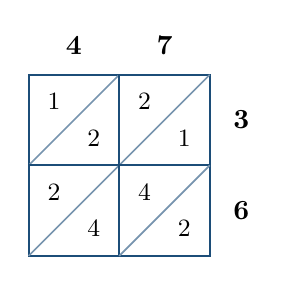
\begin{tikzpicture}[scale=1.15]
        \lgrid{2}{2}
        \ltop{1}{4}\ltop{2}{7}\lside{2}{1}{3}\lside{2}{2}{6}
        \lcell{1}{1}{1}{2}\lcell{2}{1}{2}{1}
        \lcell{1}{2}{2}{4}\lcell{2}{2}{4}{2}
      \end{tikzpicture}
    \end{column}
    \begin{column}{0.55\textwidth}
      \begin{itemize}
        \item \ealpara{Pomnóż każdą z kombinacji \ealkeytr{cyfr} w odpowiedniej komórce.}{Multiply each of the combinations of \ealkey{digits} in the relevant cell.}
        \item \ealpara{\ealkeytr{Dziesiątki} idą w lewym górnym \ealkeytr{trójkącie}, \ealkeytr{jedności} w prawym dolnym.}{\ealkey{Tens} go in the upper-left \ealkey{triangle}, \ealkey{units} in the lower-right.}
      \end{itemize}
      \begin{center}
        \small
        \begin{tabular}{ll}
          $4\times3=12$ & $\rightarrow$ \;$\boxed{1}\,/\,\boxed{2}$\\
          $7\times3=21$ & $\rightarrow$ \;$\boxed{2}\,/\,\boxed{1}$\\
          $4\times6=24$ & $\rightarrow$ \;$\boxed{2}\,/\,\boxed{4}$\\
          $7\times6=42$ & $\rightarrow$ \;$\boxed{4}\,/\,\boxed{2}$
        \end{tabular}
      \end{center}
      \vspace{4pt}
      \ealpara{Odpowiedź jednocyfrowa, taka jak $3\times2=6$, jest zapisywana jako $0/6$.}{A one-\ealkey{digit} answer such as $3\times2=6$ is written $0/6$.}
    \end{column}
  \end{columns}
\end{frame}

%=====================================================================
\begin{frame}
  \ealpara{Krok 3: \ealkeytr{dodawaj} wzdłuż \ealkeytr{przekątnych}}{Step 3: \ealkey{add} along the \ealkey{diagonals}}
  \vspace{6pt}
  \begin{columns}[c]
    \begin{column}{0.48\textwidth}
      \centering
      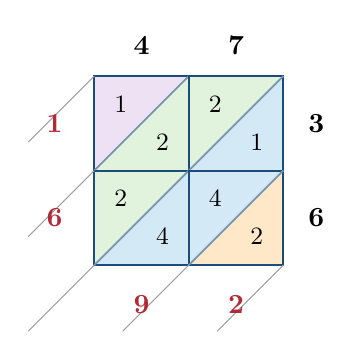
\begin{tikzpicture}[scale=1.2]
        \lband{2}{2}{3}{bandA}\lband{2}{2}{2}{bandB}
        \lband{2}{2}{1}{bandC}\lband{2}{2}{0}{bandD}
        \lgrid{2}{2}
        \draw[mmgrey!70] (0,0) -- (-0.7,-0.7);
        \draw[mmgrey!70] (0,-1) -- (-0.7,-1.7);
        \draw[mmgrey!70] (0,-2) -- (-0.7,-2.7);
        \draw[mmgrey!70] (1,-2) -- (0.3,-2.7);
        \draw[mmgrey!70] (2,-2) -- (1.3,-2.7);
        \ltop{1}{4}\ltop{2}{7}\lside{2}{1}{3}\lside{2}{2}{6}
        \lcell{1}{1}{1}{2}\lcell{2}{1}{2}{1}
        \lcell{1}{2}{2}{4}\lcell{2}{2}{4}{2}
        \lleft{1}{1}\lleft{2}{6}
        \lbot{2}{2}{1}{9}\lbot{2}{2}{2}{2}
      \end{tikzpicture}
    \end{column}
    \begin{column}{0.52\textwidth}
      \ealpara{Zacznij od prawego dolnego rogu i pracuj w górę pasów.}{Start at the bottom right and work up the strips.}
      \vspace{4pt}
      \ealpara{Wiersze: \ealkeytr{jedności}, \ealkeytr{dziesiątki}, \ealkeytr{setki}, \ealkeytr{tysiące}.}{Rows: \ealkey{units}, \ealkey{tens}, \ealkey{hundreds}, \ealkey{thousands}.}
      \begin{center}\small
      \begin{tabular}{lll}
        \cellcolor{bandA}\ealkey{units}     & $2$            & $=\hl{2}$\\
        \cellcolor{bandB}\ealkey{tens}      & $4+4+1$        & $=\hl{9}$\\
        \cellcolor{bandC}\ealkey{hundreds}  & $2+2+2$        & $=\hl{6}$\\
        \cellcolor{bandD}\ealkey{thousands} & $1$            & $=\hl{1}$\\
      \end{tabular}
      \end{center}
      \vspace{6pt}
      \begin{itemize}
        \item \ealpara{Każdy zacieniowany pas to jedna kolumna \ealkeytr{wartości pozycyjnej}.}{Each shaded strip is one \ealkey{place value} column.}
        \item \ealpara{Zapisz każdą sumę tuż poza \ealkeytr{kratą}.}{Write each total just outside the \ealkey{lattice}.}
      \end{itemize}
    \end{column}
  \end{columns}
\end{frame}

%=====================================================================
\begin{frame}
  \ealpara{Krok 4: odczytaj odpowiedź w dół po lewej i wzdłuż dołu}{Step 4: read the answer down the left and along the bottom}
  \vspace{6pt}
  \begin{columns}[c]
    \begin{column}{0.48\textwidth}
      \centering
      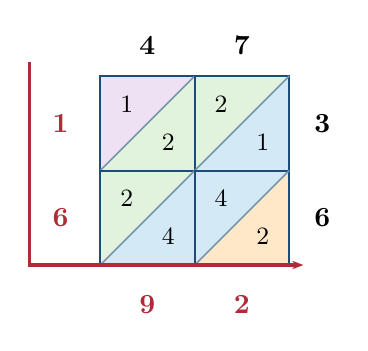
\begin{tikzpicture}[scale=1.2]
        \lband{2}{2}{3}{bandA}\lband{2}{2}{2}{bandB}
        \lband{2}{2}{1}{bandC}\lband{2}{2}{0}{bandD}
        \lgrid{2}{2}
        \ltop{1}{4}\ltop{2}{7}\lside{2}{1}{3}\lside{2}{2}{6}
        \lcell{1}{1}{1}{2}\lcell{2}{1}{2}{1}
        \lcell{1}{2}{2}{4}\lcell{2}{2}{4}{2}
        \lleft{1}{1}\lleft{2}{6}
        \lbot{2}{2}{1}{9}\lbot{2}{2}{2}{2}
        \draw[mmred,line width=1.2pt,-{Stealth[length=4pt]}]
              (-0.75,0.15) -- (-0.75,-2.0) -- (2.15,-2.0);
      \end{tikzpicture}
    \end{column}
    \begin{column}{0.52\textwidth}
      \begin{itemize}
        \item \ealpara{Czytaj w dół po lewej stronie, potem wzdłuż dołu.}{Read down the left-hand side, then along the bottom.}
        \item $1,\;6,\;9,\;2$
        \item[] \Large $47 \times 36 = \hl{1692}$
      \end{itemize}
      \vspace{8pt}
      \ealpara{Porównaj z metodą \ealkeytr{siatki}: $1200+240+210+42=1692$. to te same cztery \ealkeytr{iloczyny}, ta sama odpowiedź --- ale bez długiego dodawania.}{Compare with the \ealkey{grid} method: $1200+240+210+42=1692$. its the same four \ealkey{products}, the same answer --- but no long addition.}
    \end{column}
  \end{columns}
\end{frame}

%=====================================================================
\begin{frame}
  \ealpara{Co jeśli \ealkeytr{przekątna} \ealkeytr{dodaje} więcej niż 9?}{What if a \ealkey{diagonal} \ealkey{add}s to more than 9?}
  \vspace{6pt}
  \begin{columns}[c]
    \begin{column}{0.46\textwidth}
      \centering
      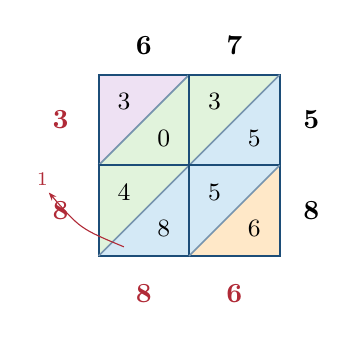
\begin{tikzpicture}[scale=1.15]
        \lband{2}{2}{3}{bandA}\lband{2}{2}{2}{bandB}
        \lband{2}{2}{1}{bandC}\lband{2}{2}{0}{bandD}
        \lgrid{2}{2}
        \ltop{1}{6}\ltop{2}{7}\lside{2}{1}{5}\lside{2}{2}{8}
        \lcell{1}{1}{3}{0}\lcell{2}{1}{3}{5}
        \lcell{1}{2}{4}{8}\lcell{2}{2}{5}{6}
        \lleft{1}{3}\lleft{2}{8}
        \lbot{2}{2}{1}{8}\lbot{2}{2}{2}{6}
        \node[mmred,font=\scriptsize] at (-0.62,-1.15) {$1$};
        \draw[mmred,-{Stealth[length=3pt]}] (0.28,-1.9) .. controls (-0.2,-1.7) .. (-0.55,-1.3);
      \end{tikzpicture}
    \end{column}
    \begin{column}{0.54\textwidth}
      \begin{center}\large $67 \times 58$\end{center}
      \vspace{4pt}
      \ealpara{Wiersze: \ealkeytr{jedności}, \ealkeytr{dziesiątki}, \ealkeytr{setki}, \ealkeytr{tysiące}. W wierszu dziesiątek: zapisz 8, \ealkeytr{przenieś} 1.}{Rows: \ealkey{units}, \ealkey{tens}, \ealkey{hundreds}, \ealkey{thousands}. In the tens row: write 8, \ealkey{carry} 1.}
      \begin{center}\small
      \begin{tabular}{lll}
        \ealkey{units}     & $6$              & $=6$\\
        \ealkey{tens}      & $5+8+5$          & $=18$ \;\hl{write 8, \ealkey{carry} 1}\\
        \ealkey{hundreds}  & $4+3+0+\hl{1}$   & $=8$\\
        \ealkey{thousands} & $3$              & $=3$\\
      \end{tabular}
      \end{center}
      \vspace{6pt}
      \begin{itemize}
        \item \ealpara{Jeśli pas sumuje się do $10$ lub więcej, zapisz cyfrę \ealkeytr{jedności} i \ealkeytr{przenieś} \ealkeytr{dziesiątki} do następnego pasa w lewo w górę.}{If a strip totals $10$ or more, write down the \ealkey{units} \ealkey{digit} and \ealkey{carry} the \ealkey{tens} into the next strip up-left.}
        \item \ealpara{Odczyt: $3,\,8,\,8,\,6$ \quad$\Rightarrow$\quad $67\times 58 = \hl{3886}$}{Reading off: $3,\,8,\,8,\,6$ \quad$\Rightarrow$\quad $67\times 58 = \hl{3886}$}
      \end{itemize}
      \vspace{2pt}
      \ealpara{\ealkeytr{Oszacowanie}: $70\times 60 = 4200$. \gd{\checkmark}}{\ealkey{Estimate}: $70\times 60 = 4200$. \gd{\checkmark}}
    \end{column}
  \end{columns}
\end{frame}

%=====================================================================
\begin{frame}
  \ealpara{Dlaczego \ealkeytr{przekątne} działają?}{Why do the \ealkey{diagonals} work?}
  \vspace{6pt}
  \begin{columns}[c]
    \begin{column}{0.44\textwidth}
      \centering
      \ealpara{Etykiety: Th = \ealkeytr{tysiące}, H = \ealkeytr{setki}, T = \ealkeytr{dziesiątki}, U = \ealkeytr{jedności}.}{Labels: Th = \ealkey{thousands}, H = \ealkey{hundreds}, T = \ealkey{tens}, U = \ealkey{units}.}
      \vspace{4pt}
      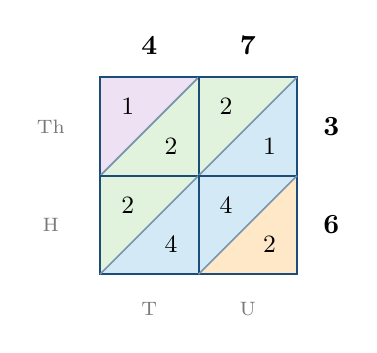
\begin{tikzpicture}[scale=1.25]
        \lband{2}{2}{3}{bandA}\lband{2}{2}{2}{bandB}
        \lband{2}{2}{1}{bandC}\lband{2}{2}{0}{bandD}
        \lgrid{2}{2}
        \ltop{1}{4}\ltop{2}{7}\lside{2}{1}{3}\lside{2}{2}{6}
        \lcell{1}{1}{1}{2}\lcell{2}{1}{2}{1}
        \lcell{1}{2}{2}{4}\lcell{2}{2}{4}{2}
        \node[font=\scriptsize,mmgrey] at (-0.5,-0.5) {Th};
        \node[font=\scriptsize,mmgrey] at (-0.5,-1.5) {H};
        \node[font=\scriptsize,mmgrey] at (0.5,-2.35) {T};
        \node[font=\scriptsize,mmgrey] at (1.5,-2.35) {U};
      \end{tikzpicture}
    \end{column}
    \begin{column}{0.56\textwidth}
      \begin{itemize}
        \item \ealpara{Lewa górna komórka naprawdę oznacza $40\times 30 = 1200$, tj. \hl{12} \ealkeytr{setek}.}{The top-left cell really means $40\times 30 = 1200$, i.e.\ $\hl{12}$ \emph{\ealkey{hundreds}}.}
        \item \ealpara{Jej \textbf{2} leży na \ealkeytr{przekątnej} \ealkeytr{setek}, a jej \textbf{1} leży o jedną \ealkeytr{przekątną} dalej w lewo --- \ealkeytr{tysiące}. Dokładnie tak.}{Its \textbf{2} sits on the \ealkey{hundreds} \ealkey{diagonal} and its \textbf{1} sits one \ealkey{diagonal} further left --- the \ealkey{thousands}. Exactly right.}
        \item \ealpara{Każdy krok w lewo lub w górę w \ealkeytr{kracie} mnoży przez $10$; oba ruchy przesuwają cię o jedną \ealkeytr{przekątną}.}{Every step you move \emph{left} or \emph{up} in the \ealkey{lattice} multiplies by $10$; both moves shift you one \ealkey{diagonal} along.}
        \item[] \ealpara{Więc \ealkeytr{przekątna} to kolumna \ealkeytr{wartości pozycyjnej}. Dlatego zera nie są potrzebne: geometria liczy za nas.}{So a \ealkey{diagonal} is a \ealkey{place value} column. That is why the zeros are not needed: the geometry is doing the counting for us.}
      \end{itemize}
    \end{column}
  \end{columns}
\end{frame}

%=====================================================================
\begin{frame}
  \ealpara{Większa \ealkeytr{krata}: $327 \times 48$}{A bigger \ealkey{lattice}: $327 \times 48$}
  \vspace{6pt}
  \begin{columns}[c]
    \begin{column}{0.5\textwidth}
      \centering
      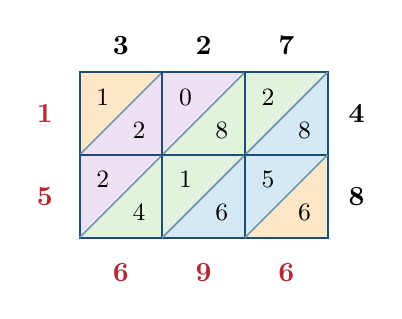
\begin{tikzpicture}[scale=1.05]
        \lband{3}{2}{4}{bandA}\lband{3}{2}{3}{bandB}
        \lband{3}{2}{2}{bandC}\lband{3}{2}{1}{bandD}
        \lband{3}{2}{0}{bandA}
        \lgrid{3}{2}
        \ltop{1}{3}\ltop{2}{2}\ltop{3}{7}
        \lside{3}{1}{4}\lside{3}{2}{8}
        \lcell{1}{1}{1}{2}\lcell{2}{1}{0}{8}\lcell{3}{1}{2}{8}
        \lcell{1}{2}{2}{4}\lcell{2}{2}{1}{6}\lcell{3}{2}{5}{6}
        \lleft{1}{1}\lleft{2}{5}
        \lbot{3}{2}{1}{6}\lbot{3}{2}{2}{9}\lbot{3}{2}{3}{6}
      \end{tikzpicture}
    \end{column}
    \begin{column}{0.5\textwidth}
      \ealpara{Wiersze: \ealkeytr{jedności}, \ealkeytr{dziesiątki}, \ealkeytr{setki}, \ealkeytr{tysiące}, \ealkeytr{dziesiątki tysięcy}.}{Rows: \ealkey{units}, \ealkey{tens}, \ealkey{hundreds}, \ealkey{thousands}, \ealkey{ten thousands}.}
      \begin{center}\small
      \begin{tabular}{lll}
        \ealkey{units}       & $6$                & $=6$\\
        \ealkey{tens}        & $5+6+8$            & $=19$ \hl{$\to$ 9, \ealkey{carry} 1}\\
        \ealkey{hundreds}    & $1+4+2+8+\hl{1}$   & $=16$ \hl{$\to$ 6, \ealkey{carry} 1}\\
        \ealkey{thousands}   & $2+0+2+\hl{1}$     & $=5$\\
        \ealkey{ten thous.}  & $1$                & $=1$\\
      \end{tabular}
      \end{center}
      \vspace{4pt}
      \begin{itemize}
        \item \ealpara{Trzy \ealkeytr{cyfry} przez dwie \ealkeytr{cyfry} $\Rightarrow$ \ealkeytr{krata} $3\times 2$.}{Three \ealkey{digits} by two \ealkey{digits} $\Rightarrow$ a $3\times 2$ \ealkey{lattice}.}
        \item \ealpara{Nic więcej się nie zmienia.}{Nothing else changes.}
        \item \large $327\times48 = \hl{15\,696}$
      \end{itemize}
    \end{column}
  \end{columns}
\end{frame}

%=====================================================================
\begin{frame}
  \ealpara{Twoja kolej: \ealkeytr{krata}}{Your turn: \ealkey{lattice}}
  \vspace{6pt}
  \begin{center}
    \begin{tabular}{lll}
      \textbf{(a)} $38\times 24 = \ablank{912}$ &\quad
      \textbf{(b)} $65\times 43 = \ablank{2795}$ &\quad
      \textbf{(c)} $57\times 89 = \ablank{5073}$\\[10pt]
      \textbf{(d)} $127\times 36 = \ablank{4572}$ &\quad
      \textbf{(e)} $408\times 57 = \ablank{23\,256}$ &\quad
      \textbf{(f)} $234\times 156 = \ablank{36\,504}$
    \end{tabular}
  \end{center}
  \vspace{14pt}
  \begin{center}
    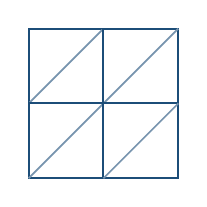
\begin{tikzpicture}[scale=0.95]
      \lgrid{2}{2}
    \end{tikzpicture}
    \hspace{26pt}
    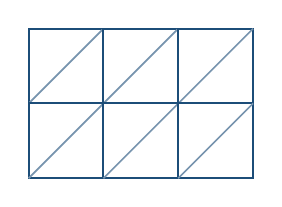
\begin{tikzpicture}[scale=0.95]
      \lgrid{3}{2}
    \end{tikzpicture}
    \hspace{26pt}
    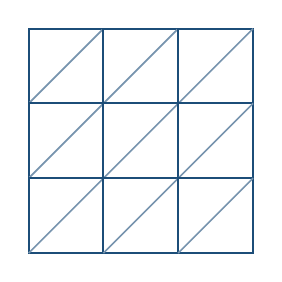
\begin{tikzpicture}[scale=0.95]
      \lgrid{3}{3}
    \end{tikzpicture}
  \end{center}
\end{frame}

%=====================================================================
\begin{frame}[plain]
  \vfill
  \centering
  \ealpara{A teraz \ealkeytr{przecinek dziesiętny}}{And now the \ealkey{decimal point}}
  \vfill
\end{frame}

%=====================================================================
\begin{frame}
  \ealpara{Najpierw: zawsze \ealkeytr{oszacowanie}}{First: always \ealkey{estimate}}
  \vspace{6pt}
  \begin{center}
    \Large $4.7 \times 3.6$
  \end{center}
  \vspace{4pt}
  \begin{center}
    \ealpara{Odpowiedź jest około $\hl{20}$. \checkmark\ jedyna blisko $20$.}{the answer is about $\hl{20}$. \checkmark\ the only one near $20$.}
    \vspace{2pt}
    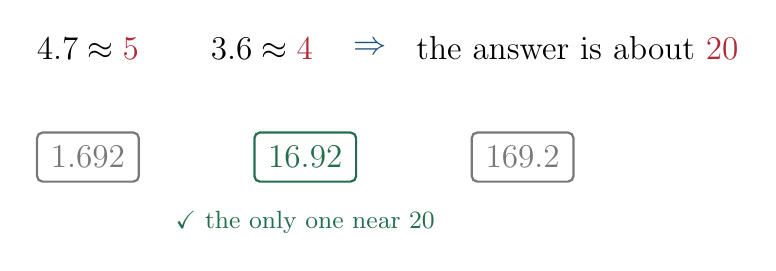
\begin{tikzpicture}[scale=0.92]
      \node[font=\large] at (0,0) {$4.7 \approx \hl{5}$};
      \node[font=\large] at (2.4,0) {$3.6 \approx \hl{4}$};
      \node[font=\large] at (3.9,0) {\textcolor{mmblue}{$\Rightarrow$}};
      \node[font=\large,anchor=west] at (4.4,0) {the answer is about $\hl{20}$};
      \foreach \x/\lab/\col in {0/$1.692$/mmgrey, 3/$16.92$/mmgreen, 6/$169.2$/mmgrey}
        {\node[draw=\col,thick,rounded corners=2pt,inner sep=5pt,text=\col,font=\large]
           at (\x,-1.5) {\lab};}
      \node[mmgreen,font=\small] at (3,-2.4) {\checkmark\ the only one near $20$};
    \end{tikzpicture}
  \end{center}
  \vspace{2pt}
  \begin{itemize}
    \item \ealpara{\ealkeytr{Krata} da \ealkeytr{cyfry} $1\,6\,9\,2$ niezależnie od tego, co robią \ealkeytr{przecinki dziesiętne}.}{\ealkey{Lattice} will give the \ealkey{digits} $1\,6\,9\,2$ whatever the \ealkey{decimal point}s are doing.}
    \item \ealpara{Musimy tylko ustalić, gdzie trafia \ealkeytr{przecinek dziesiętny}.}{We just need to work out where the \ealkey{decimal point} goes.}
  \end{itemize}
\end{frame}

%=====================================================================
\begin{frame}
  \ealpara{Zasada \ealkeytr{przecinka dziesiętnego}}{The \ealkey{decimal point} rule}
  \vspace{6pt}
  \begin{columns}[c]
    \begin{column}{0.5\textwidth}
      \centering
      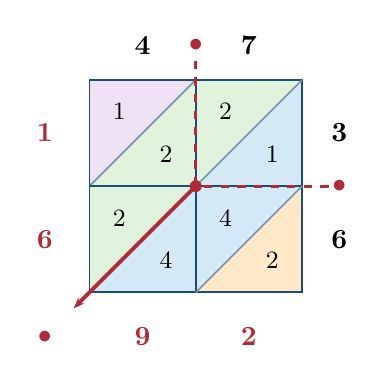
\begin{tikzpicture}[scale=1.35]
        \lband{2}{2}{3}{bandA}\lband{2}{2}{2}{bandB}
        \lband{2}{2}{1}{bandC}\lband{2}{2}{0}{bandD}
        \lgrid{2}{2}
        \ltop{1}{4}\ltop{2}{7}\lside{2}{1}{3}\lside{2}{2}{6}
        \lcell{1}{1}{1}{2}\lcell{2}{1}{2}{1}
        \lcell{1}{2}{2}{4}\lcell{2}{2}{4}{2}
        \node[mmred,font=\bfseries] at (1,0.32) {$\bullet$};
        \node[mmred,font=\bfseries] at (2.35,-1) {$\bullet$};
        \draw[mmred,dashed,line width=1pt] (1,0.18) -- (1,-1);
        \draw[mmred,dashed,line width=1pt] (2.25,-1) -- (1,-1);
        \fill[mmred] (1,-1) circle (1.6pt);
        \draw[mmred,line width=1.4pt,-{Stealth[length=4pt]}] (1,-1) -- (-0.15,-2.15);
        \lleft{1}{1}\lleft{2}{6}
        \lbot{2}{2}{1}{9}\lbot{2}{2}{2}{2}
        \node[mmred,font=\bfseries] at (-0.42,-2.42) {$\bullet$};
      \end{tikzpicture}
    \end{column}
    \begin{column}{0.5\textwidth}
      \begin{enumerate}
        \item \ealpara{Zignoruj \ealkeytr{przecinki dziesiętne} i zbuduj \ealkeytr{kratę} z \ealkeytr{cyfr}: $47$ i $36$.}{Ignore the \ealkey{decimal point}s and build the \ealkey{lattice} from the \ealkey{digits}: $47$ and $36$.}
        \item \ealpara{Zaznacz \ealkeytr{przecinek dziesiętny} górnej liczby na górnej krawędzi, a liczby bocznej na prawej krawędzi.}{Mark the \ealkey{decimal point} of the top number on the top edge, and of the side number on the right edge.}
        \item \ealpara{Przesuń jeden w dół, a drugi w poprzek, aż się spotkają.}{Slide one \emph{down} and the other \emph{across} until they \hl{meet}.}
        \item \ealpara{Od tego punktu spotkania podążaj \ealkeytr{przekątną} w lewo w dół, aż opuścisz \ealkeytr{kratę}. Tam trafia \ealkeytr{przecinek dziesiętny} w odpowiedzi.}{From that meeting point, \hl{follow the \ealkey{diagonal}} down-left until you leave the \ealkey{lattice}. That is where the \ealkey{decimal point} goes in the answer.}
      \end{enumerate}
      \vspace{6pt}
      \begin{center}\large $4.7\times 3.6 = \hl{16.92}$\end{center}
      \ealpara{\ealkeytr{Oszacowanie} było $20$. \gd{\checkmark}}{\ealkey{Estimate} was $20$. \gd{\checkmark}}
    \end{column}
  \end{columns}
\end{frame}

%=====================================================================
\begin{frame}
  \ealpara{Ta sama \ealkeytr{krata}, inny \ealkeytr{przecinek dziesiętny}}{Same \ealkey{lattice}, different \ealkey{decimal point}}
  \vspace{6pt}
  \begin{columns}[c]
    \begin{column}{0.5\textwidth}
      \centering
      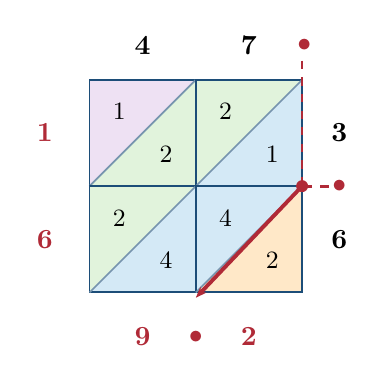
\begin{tikzpicture}[scale=1.35]
        \lband{2}{2}{3}{bandA}\lband{2}{2}{2}{bandB}
        \lband{2}{2}{1}{bandC}\lband{2}{2}{0}{bandD}
        \lgrid{2}{2}
        \ltop{1}{4}\ltop{2}{7}\lside{2}{1}{3}\lside{2}{2}{6}
        \lcell{1}{1}{1}{2}\lcell{2}{1}{2}{1}
        \lcell{1}{2}{2}{4}\lcell{2}{2}{4}{2}
        \node[mmred,font=\bfseries] at (2.02,0.32) {$\bullet$};
        \node[mmred,font=\bfseries] at (2.35,-1) {$\bullet$};
        \draw[mmred,dashed,line width=1pt] (2,0.18) -- (2,-1);
        \draw[mmred,dashed,line width=1pt] (2.25,-1) -- (2,-1);
        \fill[mmred] (2,-1) circle (1.6pt);
        \draw[mmred,line width=1.4pt,-{Stealth[length=4pt]}] (2,-1) -- (1,-2.05);
        \lleft{1}{1}\lleft{2}{6}
        \lbot{2}{2}{1}{9}\lbot{2}{2}{2}{2}
        \node[mmred,font=\bfseries] at (1,-2.42) {$\bullet$};
      \end{tikzpicture}
    \end{column}
    \begin{column}{0.5\textwidth}
      \begin{center}\Large $47 \times 3.6$\end{center}
      \vspace{4pt}
      \begin{itemize}
        \item \ealpara{$47$ nie ma zapisanego \ealkeytr{przecinka dziesiętnego}, więc znajduje się na skrajnej prawej górnej krawędzi.}{$47$ has no \ealkey{decimal point} written, so it sits at the \textbf{far right} of the top edge.}
        \item \ealpara{$3.6$ umieszcza swój przecinek między dwoma wierszami, jak poprzednio.}{$3.6$ puts its point between the two rows, as before.}
        \item \ealpara{Spotykają się niżej, więc \ealkeytr{przekątna} opuszcza \ealkeytr{kratę} o jedno miejsce dalej w prawo.}{They meet lower down, so the \ealkey{diagonal} leaves the \ealkey{lattice} one place further right.}
      \end{itemize}
      \vspace{6pt}
      \begin{center}\large $47\times 3.6 = \hl{169.2}$\end{center}
      \vspace{4pt}
      \ealpara{\ealkeytr{Oszacowanie}: $50\times 4 = 200$. \gd{\checkmark} \ealkeytr{Cyfry} w \ealkeytr{kracie} nigdy się nie zmieniły: $1\,6\,9\,2$. Tylko przecinek się przesunął.}{\ealkey{Estimate}: $50\times 4 = 200$. \gd{\checkmark} The \ealkey{lattice} \ealkey{digits} never changed: $1\,6\,9\,2$. Only the point moved.}
    \end{column}
  \end{columns}
\end{frame}

%=====================================================================
\begin{frame}
  \ealpara{Szybka kontrola: policz \ealkeytr{miejsca dziesiętne}}{The quick check: count the \ealkey{decimal place}s}
  \vspace{6pt}
  \begin{center}
    \ealpara{Policz \ealkeytr{miejsca dziesiętne}.}{Count the \ealkey{decimal place}s.}
    \vspace{4pt}
    \begin{tabular}{lcl}
      $4.7\times 3.6$  & $1+1 = 2$ places & $\Rightarrow$ $16\hl{.}92$\\
      $47\times 3.6$   & $0+1 = 1$ place  & $\Rightarrow$ $169\hl{.}2$\\
      $0.47\times 3.6$ & $2+1 = 3$ places & $\Rightarrow$ $1\hl{.}692$\\
      $0.47\times 0.36$& $2+2 = 4$ places & $\Rightarrow$ $0\hl{.}1692$\\
    \end{tabular}
  \end{center}
  \vspace{10pt}
  \begin{itemize}
    \item \ealpara{\ealkeytr{Cyfry} $1692$ pochodzą z tej samej \ealkeytr{kraty} za każdym razem.}{The \ealkey{digits} $1692$ come from the same \ealkey{lattice} every single time.}
    \item \ealpara{Całkowita liczba \ealkeytr{miejsc dziesiętnych} w pytaniu $=$ \ealkeytr{miejsca dziesiętne} w odpowiedzi.}{Total \ealkey{decimal place}s in the question $=$ \ealkey{decimal place}s in the answer.}
    \item \ealpara{Zasada \ealkeytr{przekątnej} i zasada liczenia zawsze się zgadzają --- użyj tej, którą wolisz, i sprawdź z \ealkeytr{oszacowaniem}.}{The \ealkey{diagonal} rule and the counting rule always agree --- use whichever you prefer, and \emph{check against your \ealkey{estimate}}.}
  \end{itemize}
  \vspace{6pt}
  \ealpara{Uważaj na (d): po policzeniu czterech \ealkeytr{miejsc dziesiętnych} potrzebujesz \ealkeytr{zera wiodącego}, aby wypełnić lukę.}{Careful with (d): after counting four \ealkey{decimal place}s you need a \ealkey{leading zero} to fill the gap.}
\end{frame}

%=====================================================================
\begin{frame}
  \ealpara{Rozwiązany przykład: $12.5 \times 3.4$}{Worked example: $12.5 \times 3.4$}
  \vspace{6pt}
  \begin{columns}[c]
    \begin{column}{0.5\textwidth}
      \centering
      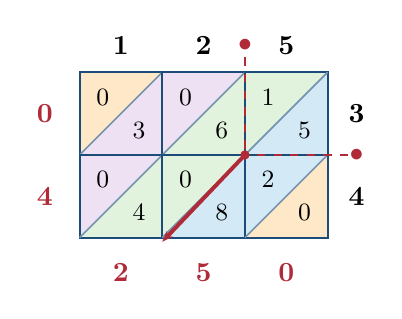
\begin{tikzpicture}[scale=1.05]
        \lband{3}{2}{4}{bandA}\lband{3}{2}{3}{bandB}
        \lband{3}{2}{2}{bandC}\lband{3}{2}{1}{bandD}
        \lband{3}{2}{0}{bandA}
        \lgrid{3}{2}
        \ltop{1}{1}\ltop{2}{2}\ltop{3}{5}
        \lside{3}{1}{3}\lside{3}{2}{4}
        \lcell{1}{1}{0}{3}\lcell{2}{1}{0}{6}\lcell{3}{1}{1}{5}
        \lcell{1}{2}{0}{4}\lcell{2}{2}{0}{8}\lcell{3}{2}{2}{0}
        \node[mmred,font=\bfseries] at (2,0.32) {$\bullet$};
        \node[mmred,font=\bfseries] at (3.35,-1) {$\bullet$};
        \draw[mmred,dashed,line width=1pt] (2,0.18) -- (2,-1);
        \draw[mmred,dashed,line width=1pt] (3.25,-1) -- (2,-1);
        \fill[mmred] (2,-1) circle (1.6pt);
        \draw[mmred,line width=1.4pt,-{Stealth[length=4pt]}] (2,-1) -- (1,-2.05);
        \lleft{1}{0}\lleft{2}{4}
        \lbot{3}{2}{1}{2}\lbot{3}{2}{2}{5}\lbot{3}{2}{3}{0}
      \end{tikzpicture}
    \end{column}
    \begin{column}{0.5\textwidth}
      \ealpara{Wiersze: \ealkeytr{jedności}, \ealkeytr{dziesiątki}, \ealkeytr{setki}, \ealkeytr{tysiące}, \ealkeytr{dziesiątki tysięcy}.}{Rows: \ealkey{units}, \ealkey{tens}, \ealkey{hundreds}, \ealkey{thousands}, \ealkey{ten thousands}.}
      \begin{center}\small
      \begin{tabular}{lll}
        \ealkey{units}      & $0$                & $=0$\\
        \ealkey{tens}       & $2+8+5$            & $=15$ \hl{$\to$ 5, \ealkey{carry} 1}\\
        \ealkey{hundreds}   & $0+4+1+6+\hl{1}$   & $=12$ \hl{$\to$ 2, \ealkey{carry} 1}\\
        \ealkey{thousands}  & $0+0+3+\hl{1}$     & $=4$\\
        \ealkey{ten thous.} & $0$                & $=0$\\
      \end{tabular}
      \end{center}
      \vspace{6pt}
      \begin{itemize}
        \item \ealpara{\ealkeytr{Cyfry}: $125\times 34 = 4250$.}{\ealkey{Digits}: $125\times 34 = 4250$.}
        \item \ealpara{Przecinki spotykają się po $2$ na górze i między wierszami, więc \ealkeytr{przekątna} wychodzi jedno miejsce od prawej.}{Points meet after the $2$ on top and between the rows, so the \ealkey{diagonal} exits one place from the right.}
        \item \large $12.5\times 3.4 = \hl{42.50} = \hl{42.5}$
      \end{itemize}
      \vspace{2pt}
      \ealpara{\ealkeytr{Oszacowanie}: $13\times 3 \approx 39$. \gd{\checkmark} \ealkeytr{Zero końcowe} po przecinku można pominąć.}{\ealkey{Estimate}: $13\times 3 \approx 39$. \gd{\checkmark} A \ealkey{trailing zero} after the point can be dropped.}
    \end{column}
  \end{columns}
\end{frame}

%=====================================================================
\begin{frame}
  \ealpara{Twoja kolej: \ealkeytr{ułamki dziesiętne}}{Your turn: \ealkey{decimals}}
  \vspace{6pt}
  \begin{center}
    \begin{tabular}{lll}
      \textbf{(a)} $2.4\times 3.7 = \ablank{8.88}$ &\quad
      \textbf{(b)} $6.3\times 0.8 = \ablank{5.04}$ &\quad
      \textbf{(c)} $5.2\times 4.6 = \ablank{23.92}$\\[10pt]
      \textbf{(d)} $0.46\times 2.3 = \ablank{1.058}$ &\quad
      \textbf{(e)} $13.4\times 2.5 = \ablank{33.5}$ &\quad
      \textbf{(f)} $0.85\times 0.64 = \ablank{0.544}$
    \end{tabular}
  \end{center}
  \vspace{10pt}
  \begin{center}
    \begin{minipage}{0.86\textwidth}
      \ealpara{Dla każdego zapisz swoje \ealkeytr{oszacowanie} przed rozpoczęciem.}{For each one, write your \ealkey{estimate} before you start.}
      \vspace{8pt}
      \ealpara{\textbf{Wyzwanie 1.} $1.25\times 0.48$. Dlaczego odpowiedź potrzebuje mniej \ealkeytr{cyfr} niż oczekujesz? \ablank{$=0.6$; \ealkeytr{krata} daje $6000$ i \ealkeytr{zera końcowe} znikają.}}{\textbf{Challenge 1.} $1.25\times 0.48$. Why does the answer need fewer \ealkey{digits} than you expect? \quad \ablank{$=0.6$; the \ealkey{lattice} gives $6000$ and the \ealkey{trailing zero}s disappear.}}
      \vspace{6pt}
      \ealpara{\textbf{Wyzwanie 2.} \ealkeytr{Krata} dla $\square.\square \times 4.5$ daje \ealkeytr{cyfry} $2\,7\,9\,0$ i odpowiedź $27.90$. Jaka była pierwsza liczba? \ablank{$6.2$}}{\textbf{Challenge 2.} A \ealkey{lattice} for $\square.\square \times 4.5$ gives the \ealkey{digits} $2\,7\,9\,0$ and the answer $27.90$. What was the first number? \quad \ablank{$6.2$}}
      \vspace{6pt}
      \ealpara{\textbf{Wyzwanie 3.} Wyjaśnij swojemu partnerowi, dlaczego \ealkeytr{przekątna} to to samo co kolumna \ealkeytr{wartości pozycyjnej}.}{\textbf{Challenge 3.} Explain to your partner why a \ealkey{diagonal} is the same thing as a \ealkey{place-value} column.}
    \end{minipage}
  \end{center}
\end{frame}

%=====================================================================
\begin{frame}
  \ealpara{Podsumowanie}{Summary}
  \vspace{6pt}
  \begin{columns}[T]
    \begin{column}{0.32\textwidth}
      \centering
      \ealpara{\ealkeytr{Pole}}{\ealkey{Area}}
      \vspace{4pt}
      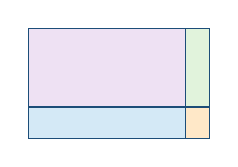
\begin{tikzpicture}[scale=0.1]
        \fill[bandD] (0,4) rectangle (20,14);\fill[bandC] (20,4) rectangle (23,14);
        \fill[bandB] (0,0) rectangle (20,4);\fill[bandA] (20,0) rectangle (23,4);
        \draw[mmblue] (0,0) rectangle (23,14);
        \draw[mmblue] (20,0)--(20,14);\draw[mmblue] (0,4)--(23,4);
      \end{tikzpicture}
      \vspace{4pt}
      \ealpara{Podziel każdą liczbę na \ealkeytr{wartości pozycyjne}; cztery \ealkeytr{pola} to cztery \ealkeytr{iloczyny}.}{Split each number into \ealkey{place value}s; the four \ealkey{areas} are the four \ealkey{products}.}
    \end{column}
    \begin{column}{0.32\textwidth}
      \centering
      \ealpara{\ealkeytr{Siatka}}{\ealkey{Grid}}
      \vspace{4pt}
      {\scriptsize\begin{tabular}{|c|c|c|}\hline
        $\times$&$40$&$7$\\\hline $30$&$1200$&$210$\\\hline $6$&$240$&$42$\\\hline
      \end{tabular}}
      \vspace{4pt}
      \ealpara{Każde zero zapisane. Niezawodne, ale na końcu długie dodawanie.}{Every zero written out. Reliable, but a long addition at the end.}
    \end{column}
    \begin{column}{0.32\textwidth}
      \centering
      \ealpara{\ealkeytr{Krata}}{\ealkey{Lattice}}
      \vspace{4pt}
      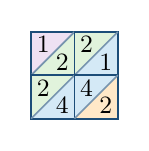
\begin{tikzpicture}[scale=0.55]
        \lband{2}{2}{3}{bandA}\lband{2}{2}{2}{bandB}
        \lband{2}{2}{1}{bandC}\lband{2}{2}{0}{bandD}
        \lgrid{2}{2}
        \lcell{1}{1}{1}{2}\lcell{2}{1}{2}{1}
        \lcell{1}{2}{2}{4}\lcell{2}{2}{4}{2}
      \end{tikzpicture}
      \vspace{4pt}
      \ealpara{Tylko \ealkeytr{cyfry}. \ealkeytr{Przekątne} \ealkeytr{przenoszą} \ealkeytr{wartość pozycyjną}. Czytaj w dół, potem w poprzek.}{\ealkey{Digits} only. The \ealkey{diagonals} \ealkey{carry} the \ealkey{place value}. Read down, then across.}
    \end{column}
  \end{columns}
  \vspace{12pt}
  \begin{center}
    \begin{minipage}{0.88\textwidth}
      \begin{itemize}
        \item \ealpara{\ealkeytr{Dziesiątki} w lewym górnym \ealkeytr{trójkącie}, \ealkeytr{jedności} w prawym dolnym.}{\ealkey{Tens} in the upper-left \ealkey{triangle}, \ealkey{units} in the lower-right.}
        \item \ealpara{\ealkeytr{Dodawaj} wzdłuż \ealkeytr{przekątnych} od prawego dolnego rogu, \ealkeytr{przenosząc} w lewo w górę.}{\ealkey{Add} down the \ealkey{diagonals} from the bottom right, \ealkey{carry}ing up-left.}
        \item \ealpara{\ealkeytr{Ułamki dziesiętne}: opuść jeden przecinek w dół, przeprowadź drugi w poprzek, a następnie podążaj \ealkeytr{przekątną} na zewnątrz. Albo policz \ealkeytr{miejsca dziesiętne}.}{\ealkey{Decimals}: drop one point down, bring the other across, then follow the \ealkey{diagonal} out. Or count the \ealkey{decimal place}s.}
        \item \ealpara{Zawsze najpierw \ealkeytr{oszacowanie}.}{Always \ealkey{estimate} first.}
      \end{itemize}
    \end{minipage}
  \end{center}
\end{frame}

\end{document}